% Bloque A - Senales y frecuencias - rama taller-senales
% Figuras: a_*.png que genera a_senales/prototipo_frecuencias.py
% Cifras: salida de ese script y resultados/a_dft_vs_fft.csv

\section{Frecuencias de trabajo}
\label{sec:senales}

\subsection{Frecuencia de muestreo y tamaño de bloque}

Se conservan los parámetros de la Tarea~1: $f_s = 16$\,kHz y bloques de
$N = 1024$ muestras con ventana Hann y 50\,\% de solapamiento. La componente
más alta que genera el emisor es la interferencia de 3500\,Hz, menos de la
mitad de la frecuencia de Nyquist ($f_s/2 = 8$\,kHz), así que ninguna se pliega
y queda margen para que el filtro de reconstrucción del emisor y el
antialiasing del receptor tengan una banda de transición amplia. El script
verifica esta condición con cada frecuencia del archivo de parámetros y se
detiene si alguna la viola.

Con $N = 1024$ la resolución es $\Delta f = f_s/N = 15{,}625$\,Hz y cada bloque
dura $N/f_s = 64$\,ms. Los tonos útiles están separados 440\,Hz, unos
28~bins, de modo que se distinguen con holgura aun con el lóbulo principal de
la ventana Hann, que ocupa 4~bins. Que $N$ sea potencia de dos permite usar la
FFT radix-2 de la Tarea~1 sin rellenar con ceros.

Los dos microcontroladores admiten esta $f_s$. El ADC de la Pico~W (RP2040,
12~bits) muestrea hasta 500\,kS/s, así que 16\,kS/s usa una fracción pequeña de
su capacidad. En el emisor, la portadora PWM de 8~bits (tope 255) oscila a
$125\,\text{MHz}/256 \approx 488$\,kHz, unas 30 veces la frecuencia de muestreo
y unas 140 veces la componente más alta, lo que facilita separarla con un
filtro RC. El reloj de muestreo sale de otra rebanada PWM con divisor 2,5:
$125\,\text{MHz}/(2{,}5 \cdot 16\,\text{kHz}) = 3125$ y
$133\,\text{MHz}/(2{,}5 \cdot 16\,\text{kHz}) = 3325$ son enteros, así que el
tope $3125-1$ (o $3325-1$) da 16\,kHz exactos con cualquiera de los dos relojes.

\subsection{Modos del emisor}

El cuadro~\ref{tab:modos} resume los tres modos. Las amplitudes relativas son
las de la Tarea~1. La salida se escala por $0{,}8/\sum_i A_i$, que es lo mismo
que calcula el emisor: si todas las componentes coincidieran en su pico la suma
valdría exactamente 0,8 del rango del PWM, y así nunca satura. Como en el
emisor todos los acumuladores de fase arrancan en cero, la referencia de Python
también usa fase cero en todas las componentes. Esta referencia es
\texttt{senal\_del\_modo()} y la usan los bloques B, C y D.

\begin{table}[H]
\centering\small
\caption{Modos del emisor. $k = f/\Delta f$ es la posición en bins con
$N = 1024$. Amplitud de salida = amplitud relativa $\times$ escala.}
\label{tab:modos}
\begin{tabular}{clrrrrc}
\toprule
Modo & Uso & $f$ (Hz) & Amp.\ relativa & Amp.\ de salida & $k$ & ¿Bin exacto? \\
\midrule
1 & prueba P1        & 440  & 1,00   & 0,800 & 28,16  & no \\
\midrule
2 & prueba P2        & 440  & 1,00   & 0,432 & 28,16  & no \\
  &                  & 880  & 0,55   & 0,238 & 56,32  & no \\
  &                  & 1320 & 0,30   & 0,130 & 84,48  & no \\
\midrule
3 & caso\_1          & 440  & 1,00   & 0,287 & 28,16  & no \\
  &                  & 880  & 0,55   & 0,158 & 56,32  & no \\
  &                  & 1320 & 0,30   & 0,086 & 84,48  & no \\
  & (interferencia)  & 3500 & 0,9373 & 0,269 & 224,00 & sí \\
\bottomrule
\end{tabular}
\end{table}

Ningún tono útil cae en un bin exacto. Un bloque de 1024 muestras no contiene un
número entero de periodos de estas componentes, y al repetirlo la FFT ve un
salto en los bordes que reparte la energía en muchos bins (fuga espectral). Con
ventana rectangular los lóbulos laterales empiezan en $-13$\,dB y caen
despacio, así que la fuga de 440\,Hz taparía los tonos más débiles. La ventana
Hann lleva la señal a cero en los bordes: su primer lóbulo lateral está en
$-31$\,dB y los siguientes caen 18\,dB por octava. A cambio, el lóbulo principal
se ensancha a 4~bins y el pico puede perder hasta 1,4\,dB cuando el tono cae
entre dos bins. Con la separación de 28~bins entre tonos, ese costo no afecta.
La interferencia de 3500\,Hz cae exactamente en el bin 224.

\paragraph{SNR del modo 3.} Las componentes tienen frecuencias distintas y son
ortogonales, así que la potencia de cada una es $A^2/2$ y las potencias se
suman. Los tres tonos útiles suman
$P_u = (1^2 + 0{,}55^2 + 0{,}3^2)/2 = 0{,}69625$ y la interferencia
$P_r = 0{,}9373^2/2 = 0{,}43927$, de donde
$\text{SNR} = 10\log_{10}(P_u/P_r) = 2{,}0004$\,dB, la misma que el
\texttt{caso\_1} (2\,dB). La amplitud exacta sería 0,937341; el redondeo a cuatro
decimales mueve la SNR menos de 0,001\,dB. La escala común del emisor multiplica
todas las componentes por el mismo factor y no cambia la SNR.

\subsection{Espectros esperados}

La figura~\ref{fig:espectros} muestra el espectro de un bloque de cada modo
antes y después de cuantizar a los 8~bits del PWM. Las magnitudes están
corregidas por la ganancia de la ventana, así que un tono de amplitud $A$ sale
en $20\log_{10}A$ cuando cae en un bin exacto. El tono de 3500\,Hz (bin 224)
sale en $-11{,}40$\,dB, igual a $20\log_{10}0{,}269$. Los tonos que caen entre
bins salen un poco más bajos por la pérdida de la Hann: 440\,Hz (bin 28,16)
pierde 0,14\,dB y 1320\,Hz (bin 84,48, casi a medio bin) pierde 1,3\,dB.

Con un paso $\Delta = 2/2^8$ y error uniforme, la potencia del ruido de
cuantización es $\Delta^2/12$. Frente a un seno de amplitud completa eso da una
SNR de $6{,}02\cdot 8 + 1{,}76 = 49{,}9$\,dB. En el espectro ese ruido se
reparte entre los bins: con $N = 1024$ y el ancho de banda equivalente de la
ventana Hann (1,5~bins), cada bin recibe $10\log_{10}(N/(2\cdot 1{,}5)) =
25{,}3$\,dB menos, y el piso por bin queda en $-75{,}3$\,dB. Las curvas ideal y
cuantizada coinciden en los picos; lo que cambia es el fondo lejos de los tonos,
que sube de menos de $-100$\,dB a cerca del piso teórico.

El error de cuantización no es exactamente ruido blanco. La señal es periódica
(440, 880 y 1320\,Hz se repiten juntas cada 400 muestras) y el error también,
así que se concentra en líneas en lugar de repartirse parejo. El caso extremo es
el modo~1, con un solo tono: la mediana del fondo queda en $-87$\,dB, pero
algunas líneas llegan a $-61$\,dB. Aun así quedan casi 60\,dB por debajo del
tono, y en los modos 2 y 3 ninguna línea pasa de $-63$\,dB. Un ADC ideal de
12~bits tendría un piso 24\,dB más bajo, así que en principio domina la
cuantización del emisor. El ADC real del RP2040 tiene menos bits efectivos que
12, y conviene medirlo en el receptor.

Esta referencia no modela el truncamiento de fase del DDS, que indexa una tabla
de 256 muestras con los 8~bits altos del acumulador. Ese truncamiento agrega
espurios propios que el bloque~C debe medir en la salida real
(sección~\ref{sec:emisor}). Para que la comparación muestra a muestra tenga
sentido, el emisor debe pasar de $[-1,1)$ al nivel PWM igual que
\texttt{cuantizar()}: $\text{nivel} = \text{round}(128\,x) + 128$, limitado
a 0--255.

\begin{figure}[H]
\centering
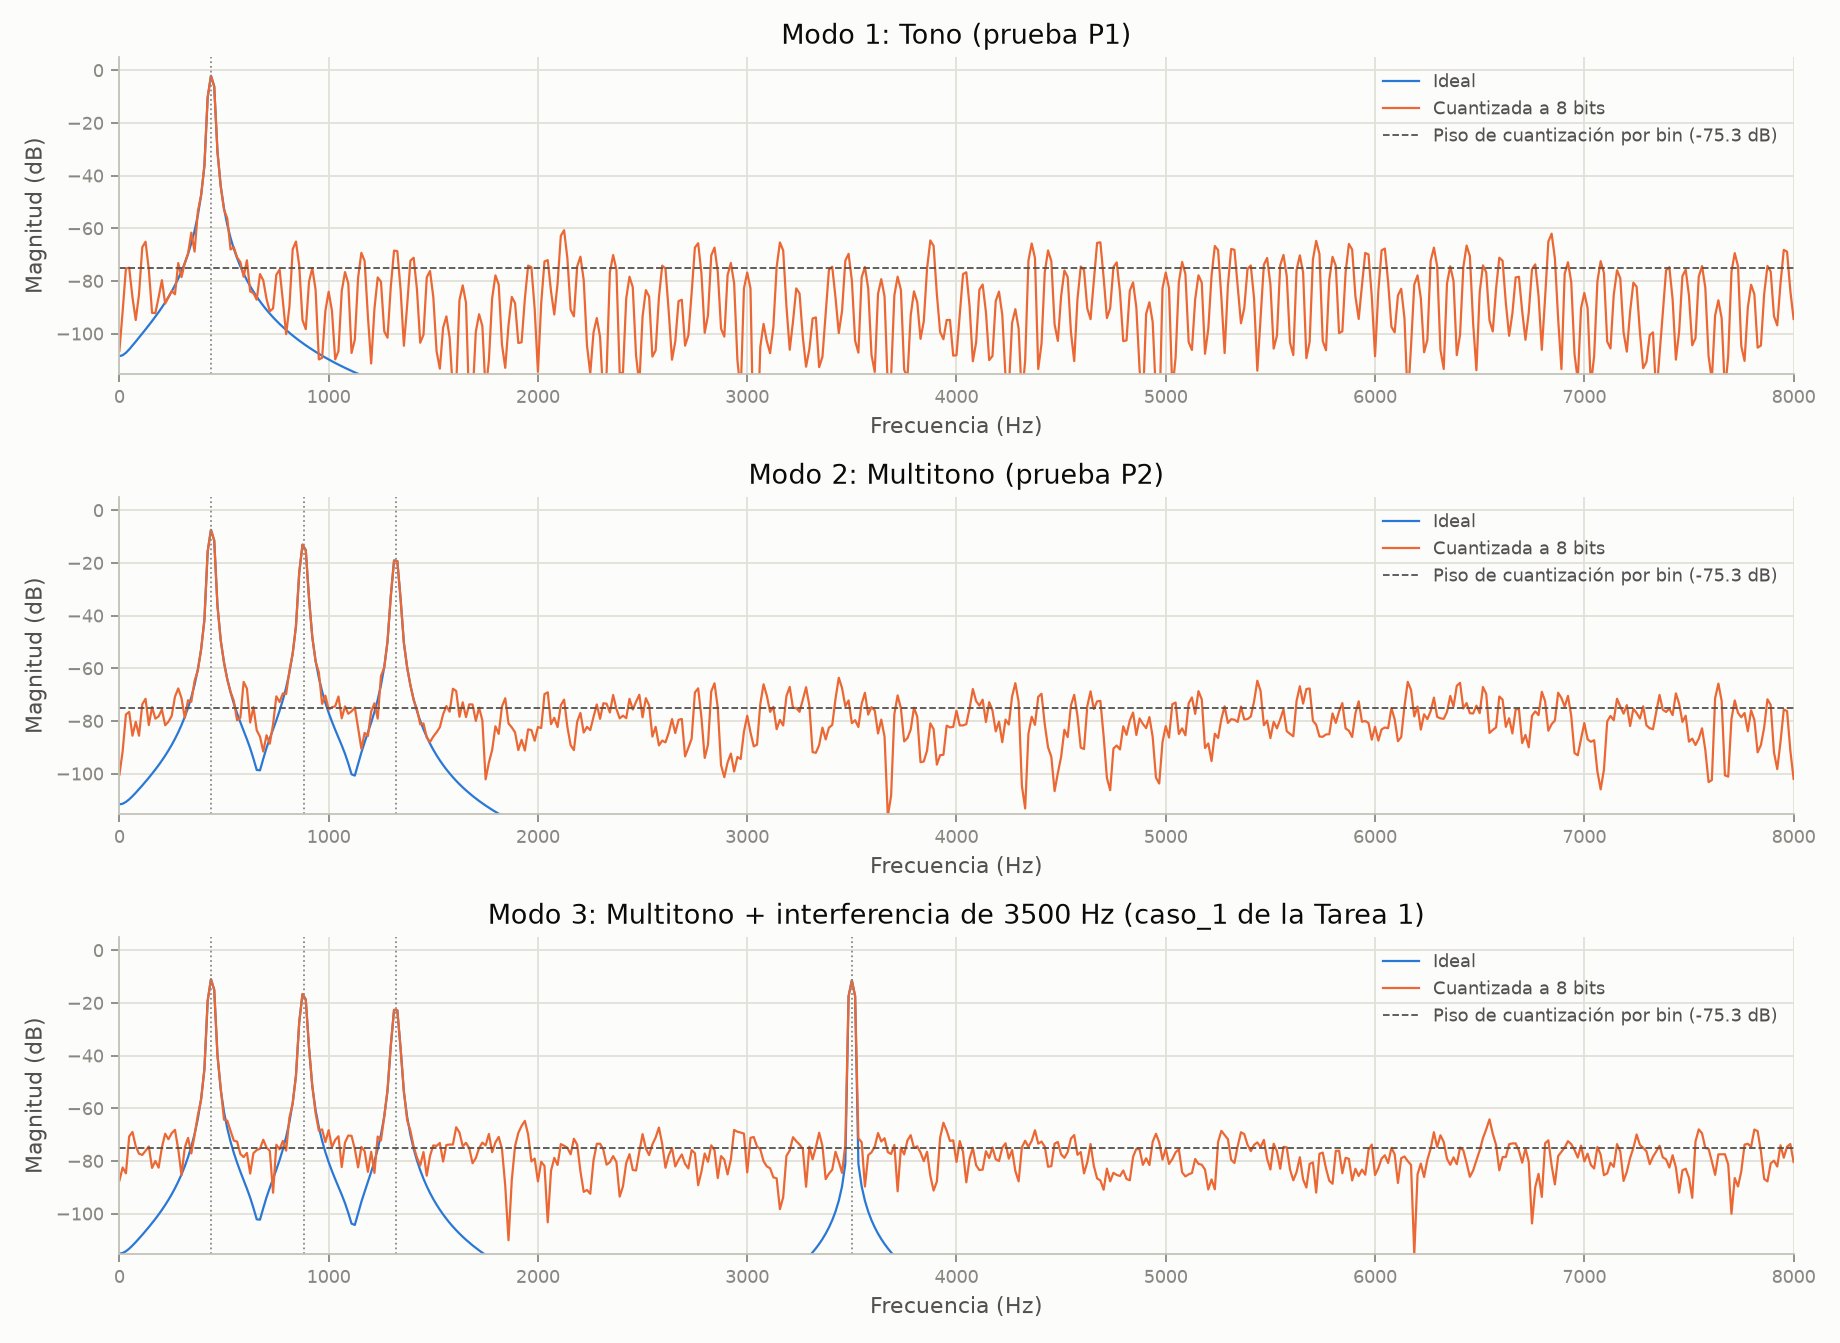
\includegraphics[width=\linewidth]{a_espectros_modos.png}
\caption{Espectro de un bloque ($N = 1024$, ventana Hann) de cada modo del
emisor, ideal y cuantizado a 8~bits. Las líneas punteadas verticales marcan las
frecuencias esperadas y la horizontal, el piso teórico de cuantización por bin.}
\label{fig:espectros}
\end{figure}

\subsection{DFT frente a FFT}

El cuadro~\ref{tab:dft_fft} compara la DFT por definición (\texttt{dft()},
dos lazos explícitos) y la FFT radix-2 iterativa (\texttt{fft()}) de
\texttt{src/dft\_fft.py}, con un bloque del modo~3 de $N = 1024$ muestras. El
tiempo es el promedio de 3 corridas de la DFT y de 50 de la FFT, en Python y en
la computadora de desarrollo. Los valores absolutos dependen de la máquina; la
razón entre ellos depende mucho menos.

\begin{table}[H]
\centering\small
\caption{DFT por definición frente a FFT radix-2 con $N = 1024$.}
\label{tab:dft_fft}
\begin{tabular}{lrr}
\toprule
 & DFT & FFT \\
\midrule
Multiplicaciones complejas & $N^2 = 1\,048\,576$ & $\tfrac{N}{2}\log_2 N = 5120$ \\
Tiempo promedio            & 858\,ms             & 4,06\,ms \\
\midrule
Razón medida / teórica     & \multicolumn{2}{c}{212 / 205} \\
Error máximo $|X_\text{DFT} - X_\text{FFT}|$ & \multicolumn{2}{c}{$4{,}0\times10^{-11}$} \\
\bottomrule
\end{tabular}
\end{table}

La aceleración medida (212 veces) coincide con la teórica
($2N/\log_2 N = 205$). No es idéntica porque el tiempo no es solo de
multiplicaciones: la DFT también evalúa una exponencial compleja por término, y
la FFT resuelve cada etapa con operaciones vectoriales de NumPy. El error máximo es $4\times 10^{-11}$ cuando el bin más
grande vale 141, un error relativo cercano a $3\times10^{-13}$, que es
redondeo de punto flotante. Las dos dan el mismo resultado. En el
microcontrolador la diferencia decide si el sistema es viable: cada bloque de
64\,ms exige 5120 multiplicaciones complejas con la FFT frente a más de un
millón con la DFT.
